\documentclass[hidelinks]{ferseminar}
\student{David Emanuel Lukšić}
\email{david-emanuel.luksic@fer.hr}
\voditelj{prof.~dr.~sc.~Željka Mihajlović}
\mjestodatum{Zagreb}{svibanj}{2018}
\naslov{Digitalna holografija u mikroskopiji}
\sazetak{Ovaj seminar sadrži kratki uvod u digitalnu holografiju i njenu primjenu u mikroskopiji. Sažeto opisuje što su hologrami, kako ih generirati i rekonstruirati na računalu. Zatim to znanje primjenjujemo u izradi jednostavnog holografskog mikroskopa i programskog rješenja za rekonstrukciju u stvarnom vremenu na GPU. Mikroskop se sastoji od web kamere rezolucije $640$x$480$, infracrvenog lasera valne duljine $780nm$ (iz CD pisača) i stalka. Ostvarena rezolucija mikroskopa je oko $10\mu{m}$.}
\begin{document}
\umetninaslov

\section{Uvod}
\lettrine[nindent=0em,lines=2]{H}olografiju (grč. \textit{hólos}, "čitav, potpun, sav" + \textit{gráfos}, "pišem, crtam") je izumio Denis Gabor 1948. godine kao način zapisa i rekonstrukcije polja valne prirode. U početku, Gabor je eksperimentirao s elektronskim mikroskopom i snimao valne fronte elektrona \cite{gabor1948new}, no pojavom prvih LASER-a snimljeni su prvi hologrami na fotografskoj ploči (E. Leith i J. Upatnieks, 1965. \cite{leith1965microscopy}). Time je holografija postala metoda snimanja i reproduciranja trodimenzionalnih slika (holograma). Hologram, za razliku od fotografije, uz amplitudu svetlosnih valova zapisuje i njihovu fazu, što omogućuje fokusiranje na različite elemente slike nakon što smo snimili hologram. Ova činjenica osnovna je prednost digitalnog holografskog mikroskopa (DHM) nad optičkim. To znači da je, teoretski, moguće pomoću DHM-a iz jedne jedine slike rekonstruirati 3D informaciju o preparatu.

Najveće poteškoće u digitalnoj holografiji stvara rekonstrukcija fazne informacije. Senzori kamere mogu snimati samo amplitudu svjetlosti, zbog čega je potrebno kodirati fazu holograma pomoću amplitude svjetlosti, obično korištenjem referentne zrake. Tu metodu nazivamo \textit{off-axis} što je vrlo skupo jer zahtijeva profesionalne optičke elemente. U ovom radu razmatramo samo \textit{inline}, odnosno \textit{on-axis} transmisijske holograme koji fazu zanemaruju. Nedostatak ovakvog holograma je stvaranje slike blizanca (eng. \emph{twin-image}), o čemu će biti riječ u poglavlju \ref{reconstruction}.

\section{Hologram, interferencija svjetlosti}
\label{interf}
Svjetlost klasično opisujemo kao val u elektromagnetskom polju. Neka u prostoru postoji savršeni točkasti izvor svjetlosti. Oko njega će se širiti elektromagnetski valovi u obliku sfere čija (kompleksna) amplituda opada linearno s udaljenošću od izvora. Huygens-Fresnel princip kaže da svaku točku na valnoj fronti možemo promatrati kao nove točkaste izvore (eng. \emph{wavelets}) \cite{goodman2005introduction}. Kada takva fronta naiđe na prepreku (promatrani objekt), valovi novih izvora se mogu apsorbirati, reflektirati, zakasniti u fazi. Kompleksnu amplitudu nove valne fronte koja je nastala prolaskom kroz objekt označit ćemo s $A_0(x,y)$. Propagaciju rezultirajućeg vala tada možemo izračunati za svaku točku u prostoru iza objekta. Matematički, račun nove valne fronte $A$ u ravnini snimanja $\Pi_s$ udaljenu za $L$ računamo sumiranjem svih doprinosa točkastih izvora $A_0$ u ravnini objekta $\Pi_0$ pomoću Fresnel-Kirchoff formule
\begin{equation}
A(x,y)=-\frac{i}{\lambda}\iint\limits_{\Pi_0}A_0(x_0,y_0)\frac{exp(i\frac{2\pi}{\lambda}r)}{r}\,dx_0dy_0
\end{equation}
\begin{equation}
r = \sqrt{(x-x_0)^2+(y-y_0)^2+L^2}
\end{equation}
gdje je $A_0$ kompleksna amplituda u ravnini objekta, a $A$ kompleksna amplituda u ravninama iza objekta, udaljenima za parametar $L$. Pokazuje se da ovaj integral možemo zapisati kao konvoluciju $A_0$ s funkcijom $h$ koja modelira širenje svjetlosti točkastog izvora (eng. \textit{point spread function}) na neku udaljenost $L$

\begin{equation}
A(x,y)=A_0\ast h_L
\end{equation}
\begin{equation}
h_L=-\frac{i}{\lambda}\frac{exp(i\frac{2\pi}{\lambda}r)}{r}
\end{equation}

Konvolucija bi bila prespora za direktnu implementaciju. Zato konvoluciju radimo u frekvencijskoj domeni (Fourierovim transformacijama). Prisjetimo se da je Fourierova transformacija konvolucije jednaka umnošku Fourierovih transformacija
\begin{equation}
\mathcal{F}(A_0\ast h_L)=\mathcal{F}(A_0)\mathcal{F}(h_L)
\end{equation}
dodatno, $\mathcal{F}(h_L)$ se može izraziti analitički, što daje bolju numeričku stabilnost
\begin{equation}
\label{propagator}
\mathcal{F}(h_L)=exp(-i\frac{2\pi}{\lambda}L\sqrt{1-\lambda^2k_x^2-\lambda^2k_y^2})
\end{equation}
gdje su $k_x$ i $k_y$ prostorne frekvencije (koordinate u frekvencijskoj domeni). Konačno izraz za propagaciju valne fronte za neku udaljenost $L$ jest
\begin{equation}
\label{angspecmeth}
A(x,y)=\mathcal{F}^{-1}(\mathcal{F}(A_0)\mathcal{F}(h_L))
\end{equation}


\begin{figure}
\includegraphics[width=\columnwidth]{holgen.png}
\caption{Amplituda u ravnini objekta, $A_0$ (lijevo) i generirani hologram (desno). U centru velikog kruga uočavamo efekt Poissonove točke: u sredini sjene kružnog elementa postoji svijetla točka usljed interferencije.}
\label{simulation}
\end{figure}

\section{Računalno simulirani hologram}
Simulirati hologram svodi se na definiranje kompleksne amplitude $A_0(x,y)$ u ravnini promatranog objekta i propagiranje valne fronte na neku udaljenost $L$. Na slici \ref{simulation} lijevo, prikazan je hologram veličine 256x256 piksela. Hologram prikazuje ilustraciju preparata kojeg smo osvjetlili ravnim valom. Crni pikseli označavaju potpunu apsorpciju, dok bijeli pikseli označavaju neometan prolazak valne fronte. U memoriji, hologram je spremljen kao dvodimenzionalno polje kompleksnih brojeva (\lstinline{complex64}). Tamo gdje su pikseli bijeli, amplituda je $1\angle0$\footnote{$\angle$ označava kompleksni kut}, a tamo gdje su crni amplituda je $0\angle0$.

Kako bismo mogli propagirati taj hologram na neku udaljenost $L$, treba izračunati polje kompleksnih brojeva $\mathcal{F}(h)$ (slika \ref{propagator_img}) jednake veličine kao i hologram pomoću jednadžbe \ref{propagator}. Konačno, radimo Fourierovu transformaciju amplitude, množimo ju s $\mathcal{F}(h)$ i vratimo inverznom Fourierovom transformacijom. Rezultirajuće polje sadrži kompleksne brojeve čiji kvadrirani iznosi odgovaraju intenzitetu holograma kojeg bi snimila kamera (slika \ref{simulation} desno) na udaljenosti $L$ od objekta.

\begin{figure}
\centering
\includegraphics[width=\columnwidth/2]{propagator.jpg}
\caption{Realni dio od $\mathcal{F}(h)$. Apsolutna vrijednost svakog piksela je $1$, a faza se mijenja radijalno s udaljenošću od centra.}
\label{propagator_img}
\end{figure}

\section{Rekonstrukcija holograma i problem slike blizanca}
\label{reconstruction}
Kamera može snimiti jedino intenzitet pristigle svjetlosti na pojedini piksel senzora. Drugim riječima, kamera snima
\begin{equation}
\mathcal{I}=|A(x,y)|^2
\end{equation} 
Znamo da je $A(x,y)$ zapravo propagirana amplituda $A_0$ na neku udaljenost $L$, odnosno konvolucija s funkcijom propagacije $h_L$. Uvedemo li funkciju neprozirnosti predmeta $t(x,y)$ (eng. \emph{opacity} $A_0 = A_{ref}(1 - t(x,y))$
\begin{equation}
\mathcal{I}=|A_0*h_L|^2
=|A_{ref}(1-t)*h_L|^2
\end{equation}
Zatim podijelimo snimljeni intenzitet sa zapamćenim originalnim intenzitetom $|A_{ref}|^2$ dobivenim snimkom kroz praznu aparaturu (\emph{normalizacija})
\begin{equation}
\frac{\mathcal{I}}{|A_{ref}|^2}=|(1-t(x,y))*h_L|^2
\end{equation}
\begin{equation}
=1-t*h_L-t^**h_L^*+|t*h_L|^2
\end{equation}
Član $|t*h_L|^2$ mora biti zanemariv u odnosu na druge članove kao klasični uvjet \emph{inline} holografije \cite{denis2005twin}. Taj uvjet zadovoljen je za prozirne predmete ili predmete malih površina. Konačno, hologramom smatramo uzorak
\begin{equation}
\mathcal{\tilde{I}}\simeq-t*h_L-t^**h_L^*
\end{equation}
Fizikalno, ovo znači da zanemarivanjem fazne informacije pri rekonstrukciji dobivamo dvije slike: realnu $t*h_L$ i virtualnu $t^**h_{-L}$. Realna se nalazi na udaljenosti $L$ ispred detektora, a virtualna na udaljenosti $L$ \glqq{iza}\grqq detektora.\\
Rekonstrukcijom ovako zapisanog holograma algoritmom opisanom u poglavlju \ref{interf} dobivamo sliku koja se sastoji od dvije komponente
\begin{gather}
\mathcal{\tilde{I}}*h_{-L}\simeq-t-t^**h_{-L}*h_{-L}\\
=-t-t^**h_{-2L}
\end{gather}
Slika $t$ je oštra (u fokusu) dok je slika $t^**h_{-2L}$ nepoželjna (slika blizanca), izvan fokusa.

\begin{figure}[h]
	\includegraphics[width=\columnwidth]{holrec.png}
	\caption{Originalni hologram (lijevo) i rekonstrukcija holograma (desno). Uočavamo da rekonstrukcija sadrži fokusiranu (oštru) sliku predmeta i nepoželjnu sliku blizanca (eng. twin-image) koja je van fokusa.}
	\label{simulation}
\end{figure}

\section{Holografski mikroskop}
\subsection{Uređaj}
\begin{figure}
\centering
\includegraphics[width=\columnwidth]{shema.png}
\caption{Realizirani mikroskop i shema}
\end{figure}
Ključni elementi digitalnog \textit{inline} holografskog mikroskopa su: 
\begin{enumerate}
	\item CMOS (odnosno CCD) senzor
	\item izvor koherentne svjetlosti
	\item stalak
\end{enumerate}
Kao izvor svjetlosti najčešće se koristi laserska dioda (bez optike za kolimaciju) zbog velike koherencije emitiranih fotona. Laserske diode su skupe, pa neki radovi pokazuju uspješnu realizaciju pomoću običnih (LED) dioda, koje imaju djelomičnu koherenciju.

Realizirani mikroskop sastoji se od:
\begin{enumerate}
	\item web kamere Logitech C210, rez. 640x480
	\item infracrvenog (780nm) lasera iz CD pisača
	\item integriranog kruga LM317 u modu za konst. struju
	\item mijeh analognog fotoaparata kao stalak
\end{enumerate}
Laserska dioda obavezno se mora napajati strujom manjom od \textasciitilde120 mA (ovisno o diodi). Kad bi struja značajno prešla tu granicu, pa čak i na mikrosekundu, dioda može pregoriti. Iz tog razloga potrebno je napraviti jednostavan izvor konstantne struje pomoću integriranog kruga LM317 i nekoliko pasivnih elemenata kao na shemi (slika \ref{driver}).
\begin{figure}
\centering
\includegraphics[width=5cm]{driver.png}
\caption{Shema izvora konstantne struje pomoću integriranog kruga LM317. Napon napajanja $V_{in}$ može biti 5-12V.}
\label{driver}
\end{figure}
\subsection{Softver}
Potreban softver za rekonstrukciju u stvarnom vremenu razvijen je u programskim jezicima Python i C. U nastavku navodimo korištene biblioteke i njihovu ulogu.
\begin{description}
	\item[Numpy] - Python biblioteka za rad s poljima. Omogućava optimirano (pisano u C-u) izvođenje matematičkih operacija nad višedimenzionalnim poljima.
	\item[OpenCV] - Python biblioteka za rad s videom. U ovom radu korištene funkcije za učitavanje i pripremu nadolazećih slika iz kamere, prikaz videa na ekran i detekciju pritiska tipki.
	\item[PyCUDA] - omogućava kompajliranje CUDA k\^oda, instanciranje Numpy polja u grafičkoj memoriji i masovno paralelno izvođenje kompajliranih funkcija nad tim poljima u grafičkom procesoru.
\end{description}
Pseudokod protoka informacije od kamere do ekrana:
\lstinputlisting[style=Python]{pseudocode.py}


\section{Rezultati}
Kako bismo pokazali rad mikroskopa odabrani su uzorci: ljudska dlaka, ogrebotina na staklu i uzorak vode iz Botaničkog vrta u Zagrebu.

Ljudska dlaka (slika \ref{hair}) dana je kao referenca za određivanje veličine vidnog polja i rezolucije. Širina ljudske dlake je oko $80 \mu{m}$, stoga možemo zaključiti da je vidno polje kvadrat stranice 1.8 mm (što se poklapa s veličinom samog senzora). Također rezolucija ostvarena je barem $10 \mu{m}$, jer možemo vidjeti izbočinu na dlaci koja je \nicefrac{1}{8} širine dlake.

Ogrebotina na predmetnom staklu (slika \ref{cross}) načinjena je brusnim papirom s obje strane stakla u obliku slova "x". Na slici \ref{cross} prikazan je originalni hologram. Rekonstrukcijom iz jedne slike na različitim dubinama, u fokus možemo dovesti svaku ogrebotinu zasebno. Na taj način možemo izmjeriti da je debljina predmetnog stakalca 1.1 mm, dok je stvarna debljina 1.12 mm. Rezolucija ovako mjerene dubine je oko 0.1 mm. Profesionalni holografski mikroskopi, koji snimaju faznu informaciju, imaju dubinsku rezoluciju u nanometrima \cite{kemper2008digital}!

Konačno, snimljen je i uzorak vode iz Botaničkog vrta u Zagrebu. Na predmetnom stakalcu načinjen je mali bazenčić, napunjen uzorkom vode i pokriven pokrovnim stakalcem. Ukupna visina uzorka je 8 mm. Na snimkama iz mikroskopa moguće je vidjeti mnogo interferencijskih uzoraka vrlo sitnih mikroorganizama u gibanju. Nažalost, rezolucija mikroskopa je vrlo gruba, stoga se ti sitni mikroorganizmi skoro uopće ne vide jednom kada se na njih fokusira. Na slici \ref{org} (c) vidimo primjer fokusiranja na veću česticu u suspenziji.

\begin{figure}
	\centering
	\includegraphics[width=\columnwidth]{hair.png}
	\caption{Ljudska dlaka na predmetnom staklu. Debljina dlake je oko $80 \mu{m}$. Hologram (lijevo) i rekonstrukcija (desno).}
	\label{hair}
\end{figure}

\begin{figure}
	\centering
	\includegraphics[width=\columnwidth]{cross.png}
	\caption{Ogrebotine na predmetnom staklu. Originalni hologram (a), rekonstrukcija na dubinama 8.3 mm (b) i 9.4 mm (c). Zaključujemo debljina stakla je \textasciitilde1.1 mm (stvarna debljina je 1.12 mm).}
	\label{cross}
\end{figure}

\begin{figure}
	\centering
	\includegraphics[width=\columnwidth]{org.png}
	\caption{Uzorak vode iz Botaničkog vrta u Zagrebu. Originalni hologram (a), rekonstrukcija na dubinama: 5.2 mm (b), 7.0 mm (c), 12.2 mm (d), 13.3 mm (e) i shema preparata. Čestica na slici (c) se u stvarnosti gibala vodoravno.}
	\label{org}
\end{figure}

\section{Zaključak}
U ovom radu opisali smo što je (\emph{inline}) hologram, kako nastaje, kako ga simulirati i rekonstruirati. Zatim smo opisali kako izraditi jednostavan digitalni holografski mikroskop (DHM) koristeći lako dostupne dijelove. Razvijen je i softver za rekonstrukciju slike u stvarnom vremenu, koristeći jezike Python i C (k\^{o}d za GPU). Pokazali smo što je njime moguće promatrati i koji su mu nedostaci (slika blizanca).

Glavna prednost ovog mikroskopa je, u odnosu na klasične, mogućnost rekonstrukcije cijelog volumena preparata iz jedne snimke. Primjer takvog preparata je kretanje mikroorganizma u volumenu vode ili tok fluida (mikročestica u njemu) oko prepreke.

Profesionalni DHM-i postoje u dvije inačice: refleksijski i transmisijski. Refleksijski detektiraju reflektirane zrake od predmeta i koriste se za proučavanje finih površina i detekciju defekata, dok transmisijski detektiraju svjetlost iza preparata kao što je opisano u ovom radu. Također, profesionalni mikroskopi rade u \emph{off-axis} režimu gdje postoji odvojena referentna zraka koja se kombinira pod blagim kutem. To omogućava rekonstrukciju fazne informacije, a time i redukciju slike blizanca.
\vfill\null

\nocite{*}
\bibliographystyle{plain}
\bibliography{bazaLiterature}
\end{document}
